\documentclass[10pt]{article}

% ---------------------------------------------------------------------------
% HomeKonet — Full System Architecture Diagram
% Landscape, large-format (A2) page to accommodate every component in full
% detail: frontend, reverse proxy, backend, background workers, pgAdmin,
% database, caching/broker layer, persistent volumes, and third-party
% integrations.
% ---------------------------------------------------------------------------

\usepackage[paperwidth=58cm,paperheight=50cm,margin=1cm]{geometry}
\usepackage[table]{xcolor}
\usepackage{tikz}
\usetikzlibrary{shapes.geometric, shapes.misc, arrows.meta, positioning, fit, backgrounds, calc}
\usepackage{lmodern}
\renewcommand{\familydefault}{\sfdefault}
\usepackage{microtype}
\pagestyle{empty}

% ---------------------------------------------------------------------------
% Colour palette
% ---------------------------------------------------------------------------
\definecolor{hkgreen}{HTML}{004406}
\definecolor{hklightgreen}{HTML}{E8F2E9}
\definecolor{hkblue}{HTML}{1B4F72}
\definecolor{hklightblue}{HTML}{EAF1F8}
\definecolor{hkorange}{HTML}{9C5700}
\definecolor{hklightorange}{HTML}{FDF0E0}
\definecolor{hkgray}{HTML}{4A4A4A}
\definecolor{hklightgray}{HTML}{F2F2F2}
\definecolor{hkred}{HTML}{8B1A1A}
\definecolor{hklightred}{HTML}{FBEAEA}
\definecolor{hkpurple}{HTML}{5B2C6F}
\definecolor{hklightpurple}{HTML}{F1E9F5}

% ---------------------------------------------------------------------------
% Node styles
% ---------------------------------------------------------------------------
\tikzset{
  every node/.style={font=\tiny},
  hosttitle/.style={
    font=\LARGE\bfseries, text=hkgreen
  },
  subtitle/.style={
    font=\normalsize, text=hkgray
  },
  groupbox/.style={
    draw=hkgray, thick, dash pattern=on 6pt off 3pt, rounded corners=4pt,
    inner sep=10mm, fill=hklightgray, fill opacity=0.35, text opacity=1
  },
  groupboxlabel/.style={
    font=\bfseries\small, text=hkgray, fill=white, fill opacity=0.9,
    text opacity=1, inner sep=1.5mm, rounded corners=1.5pt
  },
  client/.style={
    rectangle, draw=hkblue, very thick, rounded corners=3pt,
    fill=hklightblue, align=left, text width=8.4cm, inner sep=3mm,
  },
  edgeservice/.style={
    rectangle, draw=hkblue, very thick, rounded corners=3pt,
    fill=hklightblue, align=left, text width=9.6cm, inner sep=3mm,
  },
  appservice/.style={
    rectangle, draw=hkgreen, very thick, rounded corners=3pt,
    fill=hklightgreen, align=left, text width=9.2cm, inner sep=3mm,
  },
  workerservice/.style={
    rectangle, draw=hkorange, very thick, rounded corners=3pt,
    fill=hklightorange, align=left, text width=7.4cm, inner sep=2.6mm,
  },
  adminservice/.style={
    rectangle, draw=hkpurple, very thick, rounded corners=3pt,
    fill=hklightpurple, align=left, text width=7.6cm, inner sep=3mm,
  },
  datastore/.style={
    cylinder, shape border rotate=90, aspect=0.25, draw=hkgray, very thick,
    fill=hklightorange, align=center, minimum height=2.6cm, minimum width=4.6cm,
    inner sep=1mm
  },
  cache/.style={
    cylinder, shape border rotate=90, aspect=0.25, draw=hkred, very thick,
    fill=hklightred, align=center, minimum height=2.6cm, minimum width=4.2cm,
    inner sep=1mm
  },
  volume/.style={
    rectangle, draw=hkgray, thick, dash pattern=on 2pt off 2pt,
    rounded corners=2pt, fill=white, align=left, text width=3.5cm,
    font=\tiny, inner sep=1.8mm
  },
  extservice/.style={
    rectangle, draw=hkgray, thick, rounded corners=2pt,
    fill=white, align=center, text width=3.15cm, font=\tiny, inner sep=2mm
  },
  flow/.style={
    -{Latex[length=3mm,width=2mm]}, thick, draw=hkgray
  },
  flowbold/.style={
    -{Latex[length=3.5mm,width=2.4mm]}, ultra thick, draw=hkblue
  },
  flowdashed/.style={
    -{Latex[length=3mm,width=2mm]}, thick, draw=hkred, dash pattern=on 4pt off 3pt
  },
  flowvolume/.style={
    -{Latex[length=2.5mm,width=1.6mm]}, thin, draw=hkgray!70, dash pattern=on 1pt off 1.5pt
  },
  edgelabel/.style={
    font=\tiny, fill=white, fill opacity=0.85, text opacity=1,
    inner sep=0.8mm, align=center
  }
}

\begin{document}
\thispagestyle{empty}

\begin{center}
  {\LARGE\bfseries\color{hkgreen} HomeKonet --- Full System Architecture}\\[2mm]
  {\normalsize\color{hkgray} Django 5 + DRF + Channels backend \textbullet{} React 18 + Vite frontend \textbullet{} Docker Compose, single-host deployment \textbullet{} External managed Postgres (Neon)}
\end{center}
\vspace{2mm}

\begin{center}
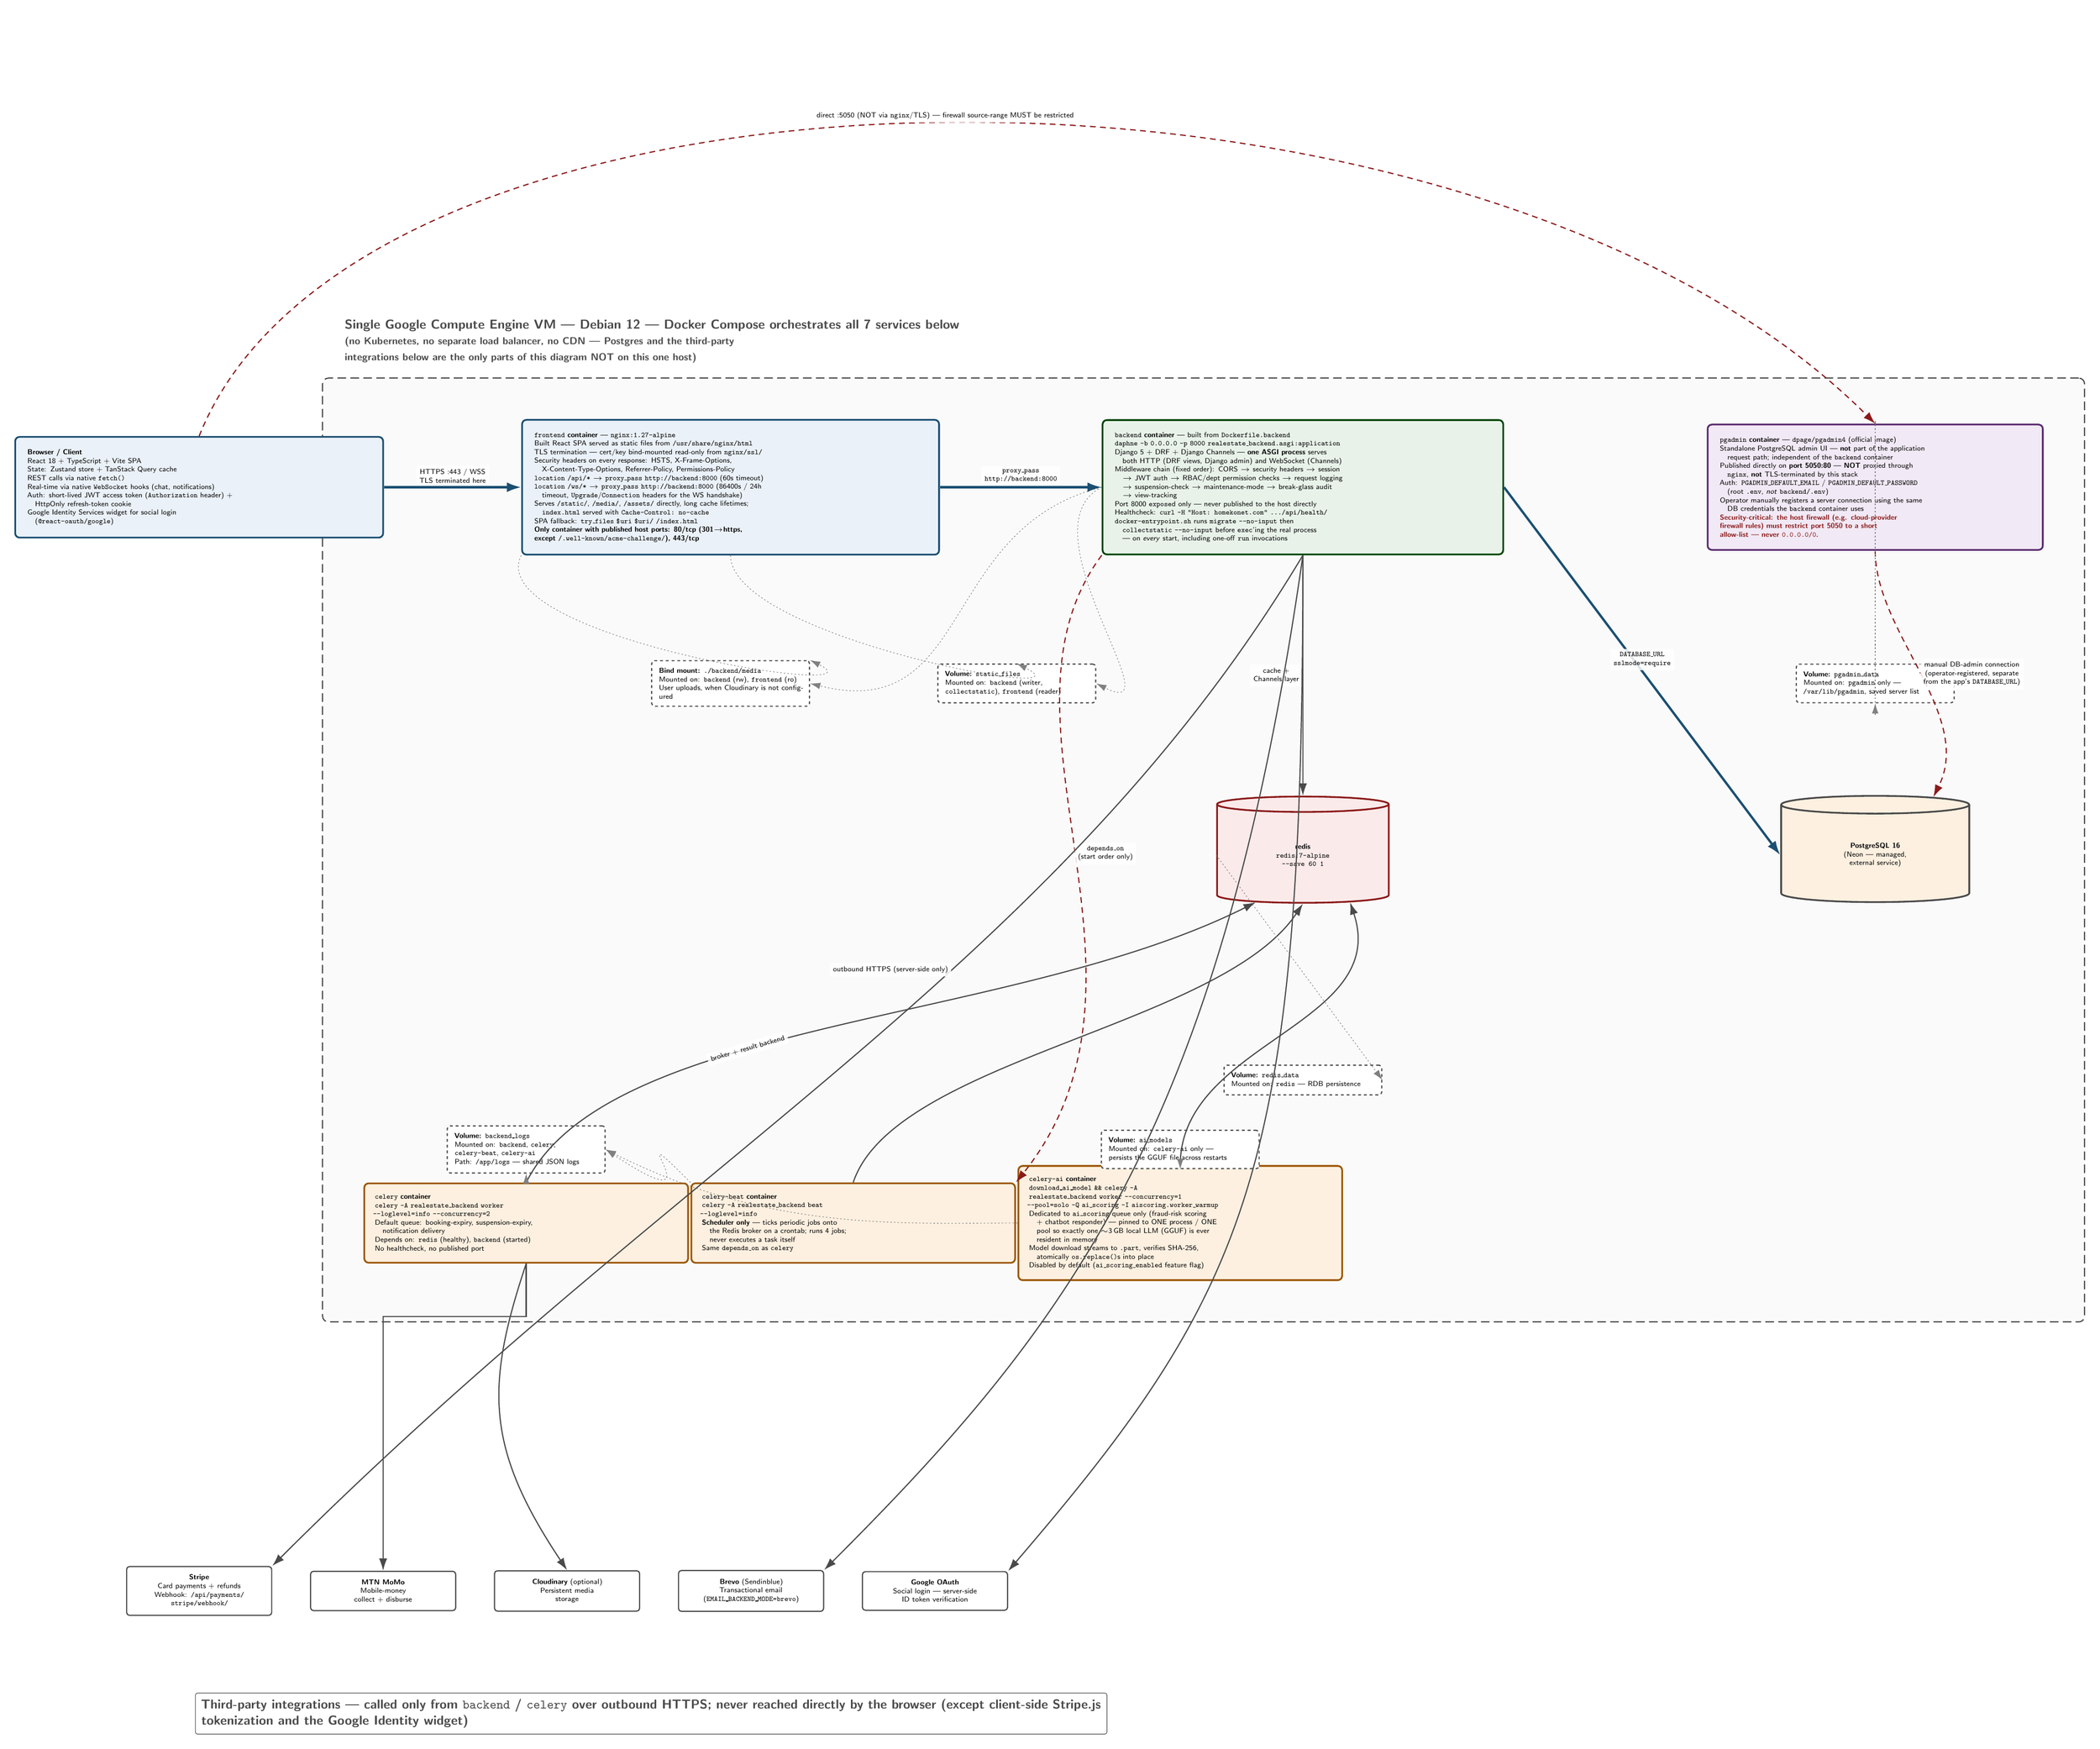
\begin{tikzpicture}[remember picture, font=\tiny]

  % =========================================================================
  % ROW A (y=18) — Client, edge, application server, pgAdmin — left to right
  % =========================================================================
  \node[client] (browser) at (-38,18) {
    \textbf{Browser / Client}\\
    React 18 + TypeScript + Vite SPA\\
    State: Zustand store + TanStack Query cache\\
    REST calls via native \texttt{fetch()}\\
    Real-time via native \texttt{WebSocket} hooks (chat, notifications)\\
    Auth: short-lived JWT access token (\texttt{Authorization} header) +\\
    \quad HttpOnly refresh-token cookie\\
    Google Identity Services widget for social login\\
    \quad (\texttt{@react-oauth/google})
  };

  \node[edgeservice] (nginx) at (-25,18) {
    \textbf{\texttt{frontend} container} --- \texttt{nginx:1.27-alpine}\\
    Built React SPA served as static files from \texttt{/usr/share/nginx/html}\\
    TLS termination --- cert/key bind-mounted read-only from \texttt{nginx/ssl/}\\
    Security headers on every response: HSTS, X-Frame-Options,\\
    \quad X-Content-Type-Options, Referrer-Policy, Permissions-Policy\\
    \texttt{location /api/*} $\rightarrow$ \texttt{proxy\_pass http://backend:8000} (60s timeout)\\
    \texttt{location /ws/*} $\rightarrow$ \texttt{proxy\_pass http://backend:8000} (86400s / 24h\\
    \quad timeout, \texttt{Upgrade}/\texttt{Connection} headers for the WS handshake)\\
    Serves \texttt{/static/}, \texttt{/media/}, \texttt{/assets/} directly, long cache lifetimes;\\
    \quad \texttt{index.html} served with \texttt{Cache-Control: no-cache}\\
    SPA fallback: \texttt{try\_files \$uri \$uri/ /index.html}\\
    \textbf{Only container with published host ports: 80/tcp (301$\to$https,}\\
    \textbf{except \texttt{/.well-known/acme-challenge/}), 443/tcp}
  };

  \node[appservice] (backend) at (-11,18) {
    \textbf{\texttt{backend} container} --- built from \texttt{Dockerfile.backend}\\
    \texttt{daphne -b 0.0.0.0 -p 8000 realestate\_backend.asgi:application}\\
    Django 5 + DRF + Django Channels --- \textbf{one ASGI process} serves\\
    \quad both HTTP (DRF views, Django admin) and WebSocket (Channels)\\
    Middleware chain (fixed order): CORS $\to$ security headers $\to$ session\\
    \quad $\to$ JWT auth $\to$ RBAC/dept permission checks $\to$ request logging\\
    \quad $\to$ suspension-check $\to$ maintenance-mode $\to$ break-glass audit\\
    \quad $\to$ view-tracking\\
    Port 8000 \texttt{expose}d only --- never published to the host directly\\
    Healthcheck: \texttt{curl -H "Host: homekonet.com" .../api/health/}\\
    \texttt{docker-entrypoint.sh} runs \texttt{migrate --no-input} then\\
    \quad \texttt{collectstatic --no-input} before \texttt{exec}'ing the real process\\
    \quad --- on \emph{every} start, including one-off \texttt{run} invocations
  };

  \node[adminservice] (pgadmin) at (3,18) {
    \textbf{\texttt{pgadmin} container} --- \texttt{dpage/pgadmin4} (official image)\\
    Standalone PostgreSQL admin UI --- \textbf{not} part of the application\\
    \quad request path; independent of the \texttt{backend} container\\
    Published directly on \textbf{port 5050:80} --- \textbf{NOT} proxied through\\
    \quad \texttt{nginx}, \textbf{not} TLS-terminated by this stack\\
    Auth: \texttt{PGADMIN\_DEFAULT\_EMAIL} / \texttt{PGADMIN\_DEFAULT\_PASSWORD}\\
    \quad (root \texttt{.env}, \emph{not} \texttt{backend/.env})\\
    Operator manually registers a server connection using the same\\
    \quad DB credentials the \texttt{backend} container uses\\
    \textcolor{hkred}{\textbf{Security-critical: the host firewall (e.g. cloud-provider}}\\
    \textcolor{hkred}{\textbf{firewall rules) must restrict port 5050 to a short}}\\
    \textcolor{hkred}{\textbf{allow-list --- never \texttt{0.0.0.0/0}.}}
  };

  % =========================================================================
  % ROW B (y=7.5) — Data / caching layer, under backend+pgAdmin
  % =========================================================================
  \node[cache] (redis) at (-11,9) {
    \textbf{redis}\\
    \texttt{redis:7-alpine}\\
    \texttt{--save 60 1}
  };

  \node[datastore] (postgres) at (3,9) {
    \textbf{PostgreSQL 16}\\
    (Neon --- managed,\\
    external service)
  };

  % =========================================================================
  % ROW C (y=-2.5) — Background workers (Celery), under Row B
  % =========================================================================
  \node[workerservice] (celery) at (-30,0) {
    \textbf{\texttt{celery} container}\\
    \texttt{celery -A realestate\_backend worker}\\
    \texttt{--loglevel=info --concurrency=2}\\
    Default queue: booking-expiry, suspension-expiry,\\
    \quad notification delivery\\
    Depends on: \texttt{redis} (healthy), \texttt{backend} (started)\\
    No healthcheck, no published port
  };

  \node[workerservice] (celerybeat) at (-22,0) {
    \textbf{\texttt{celery-beat} container}\\
    \texttt{celery -A realestate\_backend beat}\\
    \texttt{--loglevel=info}\\
    \textbf{Scheduler only} --- ticks periodic jobs onto\\
    \quad the Redis broker on a crontab; runs 4 jobs;\\
    \quad never executes a task itself\\
    Same \texttt{depends\_on} as \texttt{celery}
  };

  \node[workerservice] (celeryai) at (-14,0) {
    \textbf{\texttt{celery-ai} container}\\
    \texttt{download\_ai\_model \&\& celery -A}\\
    \texttt{realestate\_backend worker --concurrency=1}\\
    \texttt{--pool=solo -Q ai\_scoring -I aiscoring.worker\_warmup}\\
    Dedicated to \texttt{ai\_scoring} queue only (fraud-risk scoring\\
    \quad + chatbot responder) --- pinned to ONE process / ONE\\
    \quad pool so exactly one $\sim$3\,GB local LLM (GGUF) is ever\\
    \quad resident in memory\\
    Model download streams to \texttt{.part}, verifies SHA-256,\\
    \quad atomically \texttt{os.replace()}s into place\\
    Disabled by default (\texttt{ai\_scoring\_enabled} feature flag)
  };

  % =========================================================================
  % Persistent volumes — placed close to their owner(s)
  % =========================================================================
  \node[volume] (vol-redis) at (-11,3.5) {
    \textbf{Volume: \texttt{redis\_data}}\\
    Mounted on: \texttt{redis} --- RDB persistence
  };

  \node[volume] (vol-logs) at (-30,1.8) {
    \textbf{Volume: \texttt{backend\_logs}}\\
    Mounted on: \texttt{backend}, \texttt{celery},\\
    \texttt{celery-beat}, \texttt{celery-ai}\\
    Path: \texttt{/app/logs} --- shared JSON logs
  };

  \node[volume] (vol-static) at (-18,13.2) {
    \textbf{Volume: \texttt{static\_files}}\\
    Mounted on: \texttt{backend} (writer,\\
    \texttt{collectstatic}), \texttt{frontend} (reader)
  };

  \node[volume] (vol-media) at (-25,13.2) {
    \textbf{Bind mount: \texttt{./backend/media}}\\
    Mounted on: \texttt{backend} (rw), \texttt{frontend} (ro)\\
    User uploads, when Cloudinary is not configured
  };

  \node[volume] (vol-ai) at (-14,1.8) {
    \textbf{Volume: \texttt{ai\_models}}\\
    Mounted on: \texttt{celery-ai} only ---\\
    persists the GGUF file across restarts
  };

  \node[volume] (vol-pgadmin) at (3,13.2) {
    \textbf{Volume: \texttt{pgadmin\_data}}\\
    Mounted on: \texttt{pgadmin} only ---\\
    \texttt{/var/lib/pgadmin}, saved server list
  };

  % =========================================================================
  % Host boundary (drawn behind everything already placed)
  % =========================================================================
  \begin{scope}[on background layer]
    \node[groupbox, fit=(nginx)(backend)(pgadmin)(redis)(postgres)(celery)(celerybeat)
      (celeryai)(vol-redis)(vol-logs)(vol-static)(vol-media)(vol-ai)(vol-pgadmin)] (host) {};
  \end{scope}
  \node[groupboxlabel, align=left] at (host.north west) [anchor=south west, xshift=4mm, yshift=2mm] {
    Single Google Compute Engine VM --- Debian 12 --- Docker Compose orchestrates all 7 services below\\
    {\scriptsize (no Kubernetes, no separate load balancer, no CDN --- Postgres and the third-party}\\
    {\scriptsize integrations below are the only parts of this diagram NOT on this one host)}
  };

  % =========================================================================
  % ROW D (y=-13) — Third-party integrations (external, outbound only)
  % =========================================================================
  \node[extservice] (stripe) at (-38,-9) {
    \textbf{Stripe}\\
    Card payments + refunds\\
    Webhook: \texttt{/api/payments/}\\
    \texttt{stripe/webhook/}
  };
  \node[extservice] (momo) at (-33.5,-9) {
    \textbf{MTN MoMo}\\
    Mobile-money\\
    collect + disburse
  };
  \node[extservice] (cloudinary) at (-29,-9) {
    \textbf{Cloudinary} (optional)\\
    Persistent media\\
    storage
  };
  \node[extservice] (brevo) at (-24.5,-9) {
    \textbf{Brevo} (Sendinblue)\\
    Transactional email\\
    (\texttt{EMAIL\_BACKEND\_MODE=brevo})
  };
  \node[extservice] (google) at (-20,-9) {
    \textbf{Google OAuth}\\
    Social login --- server-side\\
    ID token verification
  };
  \node[groupboxlabel, draw=hkgray, fill=white] at (-38,-12) [anchor=west, xshift=-1mm] {
    \parbox{22cm}{\raggedright\textbf{Third-party integrations} --- called only from \texttt{backend} / \texttt{celery} over outbound HTTPS; \emph{never} reached directly by the browser (except client-side Stripe.js tokenization and the Google Identity widget)}
  };

  % =========================================================================
  % Arrows — request path (client to backend to data layer)
  % =========================================================================
  \draw[flowbold] (browser) -- node[edgelabel, above] {HTTPS :443 / WSS\\TLS terminated here} (nginx);
  \draw[flowbold] (nginx) -- node[edgelabel, above] {\texttt{proxy\_pass}\\\texttt{http://backend:8000}} (backend);
  \draw[flow] (backend.south) -- node[edgelabel, left] {cache +\\Channels layer} (redis.north);
  \draw[flowbold] (backend.east) -- node[edgelabel, above] {\texttt{DATABASE\_URL}\\\texttt{sslmode=require}} (postgres.west);

  % Celery workers <-> Redis broker
  \draw[flow] (celery.north) .. controls +(2,4) and +(-6,-3) .. (redis.south west)
    node[edgelabel, pos=0.4, sloped] {broker + result backend};
  \draw[flow] (celerybeat.north) .. controls +(1,3) and +(-2,-3) .. (redis.south);
  \draw[flow] (celeryai.north) .. controls +(0,3) and +(1,-3) .. (redis.south east);

  % Backend depends_on celery-family started (start order only)
  \draw[flowdashed] (backend.south west) .. controls +(-3,-4) and +(4,5) .. (celerybeat.north east)
    node[edgelabel, pos=0.5, right] {\texttt{depends\_on}\\(start order only)};

  % pgAdmin <-> Postgres (manual admin path, separate from the app connection)
  \draw[flowdashed] (pgadmin.south) .. controls +(0,-2) and +(1,2) .. (postgres.north east)
    node[edgelabel, pos=0.5, right] {manual DB-admin connection\\(operator-registered, separate\\from the app's \texttt{DATABASE\_URL})};

  % Browser direct-to-pgAdmin (out of band, security-relevant)
  \draw[flowdashed] (browser.north) .. controls +(4,10) and +(-10,10) .. (pgadmin.north)
    node[edgelabel, pos=0.5, above] {direct :5050 (NOT via \texttt{nginx}/TLS) --- firewall source-range MUST be restricted};

  % Backend / celery -> external integrations
  \draw[flow] (backend.south) .. controls +(-6,-10) and +(10,10) .. (stripe.north east)
    node[edgelabel, pos=0.4, left] {outbound HTTPS (server-side only)};
  \draw[flow] (celery.south) -- ++(0,-1.3) -| (momo.north);
  \draw[flow] (celery.south) .. controls +(-1,-3) and +(-2,3) .. (cloudinary.north);
  \draw[flow] (backend.south) .. controls +(-2,-14) and +(6,6) .. (brevo.north east);
  \draw[flow] (backend.south) .. controls +(0,-15) and +(6,7) .. (google.north east);

  % Volume attachments
  \draw[flowvolume] (redis.west) -- (vol-redis.east);
  \draw[flowvolume] (celery.north) -- (vol-logs.south);
  \draw[flowvolume] (celerybeat.north west) .. controls +(-2,2) and +(3,-2) .. (vol-logs.east);
  \draw[flowvolume] (celeryai.west) .. controls +(-3,0) and +(4,-2) .. (vol-logs.east);
  \draw[flowvolume] (backend.west) .. controls +(-2,-1) and +(2,-1) .. (vol-static.east);
  \draw[flowvolume] (nginx.south) .. controls +(0,-2) and +(2,-1) .. (vol-static.north);
  \draw[flowvolume] (nginx.south west) .. controls +(-1,-2) and +(2,-1) .. (vol-media.north east);
  \draw[flowvolume] (backend.west) .. controls +(-4,-1) and +(4,-1) .. (vol-media.east);
  \draw[flowvolume] (celeryai.north) -- (vol-ai.south);
  \draw[flowvolume] (pgadmin.north) .. controls +(0,1) and +(0,-1) .. (vol-pgadmin.south);

\end{tikzpicture}
\end{center}

\vfill
\begin{center}
\begin{minipage}{0.94\textwidth}
\scriptsize
\textbf{Legend:} \textcolor{hkblue}{Blue solid} = client/edge tier. \textcolor{hkgreen}{Green solid} = Django application server.
\textcolor{hkorange}{Orange solid} = Celery background workers. \textcolor{hkpurple}{Purple solid} = standalone admin tooling
(pgAdmin). Orange/red cylinders = external datastores (Postgres) and in-stack cache/broker (Redis).
Dashed grey boxes = persistent Docker volumes / bind mounts. \textcolor{hkblue}{Bold blue arrows} = primary
client request path. Thin grey arrows = internal broker/cache traffic. \textcolor{hkred}{Dashed red arrows} =
out-of-band / operator-only paths that bypass the normal request path (flagged where they carry
security implications). Fine dotted grey arrows = volume/bind-mount attachments.
\end{minipage}
\end{center}

\end{document}
